\documentclass{article}

% if you need to pass options to natbib, use, e.g.:
%     \PassOptionsToPackage{numbers, compress}{natbib}
% before loading neurips_2018

% ready for submission
% \usepackage{neurips_2018}

% to compile a preprint version, e.g., for submission to arXiv, add add the
% [preprint] option:
%     \usepackage[preprint]{neurips_2018}

% to compile a camera-ready version, add the [final] option, e.g.:
     \usepackage[final]{neurips_2018}

% to avoid loading the natbib package, add option nonatbib:
%     \usepackage[nonatbib]{neurips_2018}

\usepackage[utf8]{inputenc} % allow utf-8 input
\usepackage[T1]{fontenc}    % use 8-bit T1 fonts
\usepackage{hyperref}       % hyperlinks
\usepackage{url}            % simple URL typesetting
\usepackage{booktabs}       % professional-quality tables
\usepackage{amsfonts}       % blackboard math symbols
\usepackage{nicefrac}       % compact symbols for 1/2, etc.
\usepackage{microtype}      % microtypography
\usepackage{graphicx}

\title{Perceptrons vs RNNs for CPU Branch Prediction}

% The \author macro works with any number of authors. There are two commands
% used to separate the names and addresses of multiple authors: \And and \AND.
%
% Using \And between authors leaves it to LaTeX to determine where to break the
% lines. Using \AND forces a line break at that point. So, if LaTeX puts 3 of 4
% authors names on the first line, and the last on the second line, try using
% \AND instead of \And before the third author name.

\author{%
  Bandhav Veluri\\
  \texttt{bandhav@uw.edu} \\
}

\begin{document}
% \nipsfinalcopy is no longer used

\maketitle

\begin{abstract}
Branch predictors are essential pieces of hardware implemented in every modern processor. Traditionally, these are designed by analytical methods producing about 95-98\% accuracy within reasonable hardware budgets. Perceptron based predictors are proposed in literature which produce about 98\% accuracy in slightly smaller hardware footprints. In this project, I implemented perceptron and RNN based predictors for Championship Branch Prediction-1 (2004) dataset and compared the results against each other, using the classic GSHARE predictor as the baseline. I observed that RNNs are not as agile as perceptrons in being able to adapt to new program constructs and as a result, are less accurate overall.
\end{abstract}

\section{Introduction}

Modern processors are extremely complicated machines optimized to each and every gate of the hardware to extract as much cycle time as possible. As a result, processor architectures are heavily pipelined to reduce cycle time by maximizing instruction level parallelism. These deeper pipelines mean conditionally executed sections of code, such as if-else or loops, should wait for many cycles for the outcome of it's branch instruction to be evaluated. This waste of cycles is mitigated by speculatively executing conditionally executed sections and then later in the pipeline, if the speculation turns out to be wrong, pipeline is reset. This mechanism demands the speculations to be right, most of time, as resetting the pipeline is prohibitively expensive.

A branch predictor is an important part of speculative mechanisms used in modern processors to predict the address of the next instruction. They sequentially take instruction addresses as the input and if the instruction is a branch instruction, predict if the branch should be taken or not-taken. After a few cycles, the branch is actually evaluated to check if the speculation is correct. Taking the evaluated direction as the ground truth, branch predictor updates it's state accordingly.


\subsection{Branch predictors as deep learning models}

The process of continuously accepting instruction addresses, making a prediction and updating the state based on ground truth can be formulated as an online learning problem. This can be modeled as a sequential learning problem or a non-sequential learning problem by restricting the history to a fixed length. In this project, I tried both of these approaches by implementing a perceptron model and an RNN model.

\subsection{Branch prediction dataset}

I used the dataset used for Championship Branch Prediction (CBP) \url{https://www.jilp.org/cbp/}. It is one of the best datasets available for this problem with branch traces ranging from server, mobile, int and float workloads. But the data decoder exposes C++ API, so I had to write a program to dump the trace in an intermediate format for the Python model to load.

\section{Terminology and related work}

\begin{figure}
  \centering
  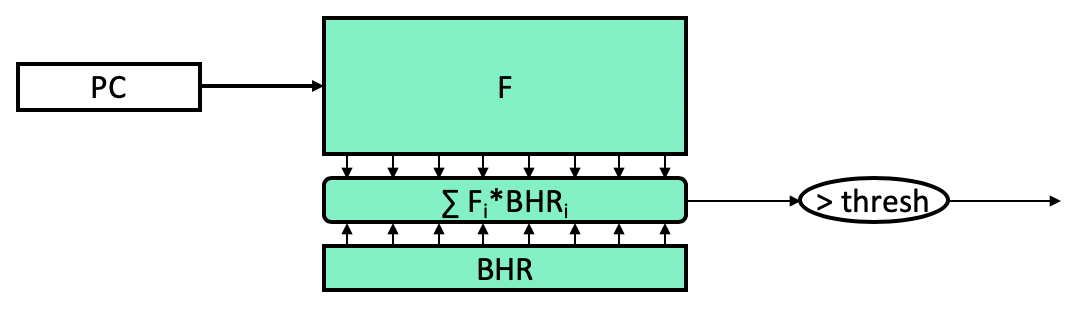
\includegraphics[width=0.7\textwidth]{perceptron.png}
  \caption{Perceptron branch predictor \cite{CezeClass}.}
  \label{fig:perceptron}
\end{figure}

Using neural networks to implement branch predictors has already been tried by \cite{Jimnez2000DynamicBP}. This work designed a predictor using a stack of perceptrons each for one instruction address. Since the total number of instruction addresses is huge, a hash of instruction address is used to access a unique perceptron. Using lower few bits of the instruction address is a decent hash. In the figure \ref{fig:perceptron}, F is a table of perceptrons addressed by the instruction address (PC). And input to the predictor is a fixed history of previous branch outcomes known as Branch History Registor (BHR). Branch outcome of the current PC is predicted based on the output of corresponding perceptron.

Branch predictors are generally evaluated using a metric called mispredicts per kilo instructions (MPKI). MPKI is the number of times the predictor has gone wrong per thousand instructions executed. This metric tells us how well the predictor did over the entire application. State-of-the-art perceptron based predictor produces really good results of about 2.8 MPKI, though we never know exact designs used in commercial processors as branch predictors are one of most closely guarded secrets by commercial processor manufacturers.

\section{Methods}
I implemented PyTorch models of perceptron and RNN branch predictors as well as a PyTorch \verb+Dataset+ for CBP workloads. CBP framework provides branch traces collected from 20 real world programs in a compressed format. I used the C++ API exposed by the CBP framework to dump branch traces in the following intermediate format suitable to be read by PyTorch \verb+Dataset+:

\begin{center}
\verb+<branch_pc> <branch_taken?> <instruction_count>+

Branch trace format
\end{center}

In the format shown above, \verb+branch_pc+ is the instruction address of this branch instruction and \verb+branch_taken?+ is it's ground truth label. Roughly, a branch prediction model would accept stream of \verb+branch_pc+s, predict branch direction for each PC and update it's internal state based on the loss computed between the predicted direction and label direction. \verb+instruction_count+ is the count of total number of instructions (branch or others) executed until this point in the program. It is just the meta data required to compute MPKI.

\subsection{Dataset}
I implemented a dataset class called \verb+BranchTraceDataset+ inheriting PyTorch's \verb+Dataset+ class. The constructor of this class takes trace file (\verb+trace_file+), BHR length (\verb+bhr_len+) and total sample size (\verb+num_samples+) as parameters. Trace file should contain branch traces in the format explained above. Objects of this class exposes an iterator which returns the tuple \verb+(pc, bhr_tensor, label_tensor, inst_count)+, corresponding to each iterator index. The length of the object would be equal to the minimum of \verb+num_samples+ and total number of lines present in the \verb+trace_file+. \verb+pc+ is the PC of the current branch instruction, \verb+bhr_tensor+ is the sequence of outcomes of past \verb+bhr_len+ branches, \verb+label_tensor+ is a binary tensor of actual branch direction and \verb+inst_count+ is the total number of instructions executed until this point.

\subsection{Perceptron Model}
The perceptron based model I implemented is same as the one shown in \ref{fig:perceptron} except for the decision making logic. I used 2-way softmax output to make the decision taken/not-taken, as opposed to threshold used in \ref{fig:perceptron}. Also, I used a table size of 512 and BHR length of 16.

\subsection{RNN model}
I tried using vanilla RNNs and GRUs with number of parameters to be around the similar range of that of Perceptron model. Upon multiple trials I found the configuration with 512 GRUs each taking BHR of width 8 as input and number of outputs equal to 2 produces best results. The two outputs of RNN model are also softmaxed to predict the branch direction.

\section{Experiments}
For each training iteration, a perceptron or RNN would be selected from the table using \verb+(pc mod table_size)+ as the index. Resulting perceptron or RNN is fed with \verb+bhr_tensor+ as the input to produce a 2-element wide \verb+output+. \verb+argmax(output)+ of the softmax output would be equal give us the predicted output. 

Loss is computed as \verb+CrossEntropyLoss(output, label_tensor)+ and the gradient of the loss is propagated back through selected perceptron or RNN. The count of mispredicts (\verb+miss_count+) is tracked on the fly by incremeting it whenever the prediction doesn't match the label, and the final MPKI score is computed as:

\begin{center}{\verb+MPKI = 1000.0 * miss_count / inst_count+}\end{center}

Following are the results obtained for all 20 workloads available in CBP dataset:

\begin{center}
\begin{tabular}{ |c|c|c| } 
 \hline
 Benchmark & Perceptron & RNN \\
 \hline
INT-1 & 8.15 & 12.477 \\
INT-2 & 8.818 & 13.133 \\
INT-3 & 14.621 & 14.921 \\
INT-4 & 3.766 & 7.675 \\
INT-5 & 0.485 & 0.68 \\
FP-1 & 3.688 & 5.121 \\
FP-2 & 1.224 & 1.316 \\
FP-3 & 0.43 & 0.521 \\
FP-4 & 0.329 & 1.679 \\
FP-5 & 1.267 & 4.922 \\
MM-1 & 8.48 & 9.029 \\
MM-2 & 10.72 & 12.833 \\
MM-3 & 4.831 & 5.759 \\
MM-4 & 2.37 & 3.545 \\
MM-5 & 5.914 & 10.571 \\
SERV-1 & 4.766 & 10.67 \\
SERV-2 & 4.877 & 10.282 \\
SERV-3 & 7.237 & 13.293 \\
SERV-4 & 5.629 & 12.676 \\
SERV-5 & 5.149 & 10.503 \\
\hline
Total & 5.137 & 8.080 \\
 \hline
\end{tabular}
\end{center}

The results over the entire dataset compared with the basline GSHARE are:

\begin{center}
\begin{tabular}{ |c|c| } 
 \hline
 Predictor & MPKI \\
 \hline
Perceptron & 5.137 \\
RNN & 8.080 \\
GSHARE & 5.301 \\
 \hline
\end{tabular}
\end{center}

\begin{figure}
  \centering
  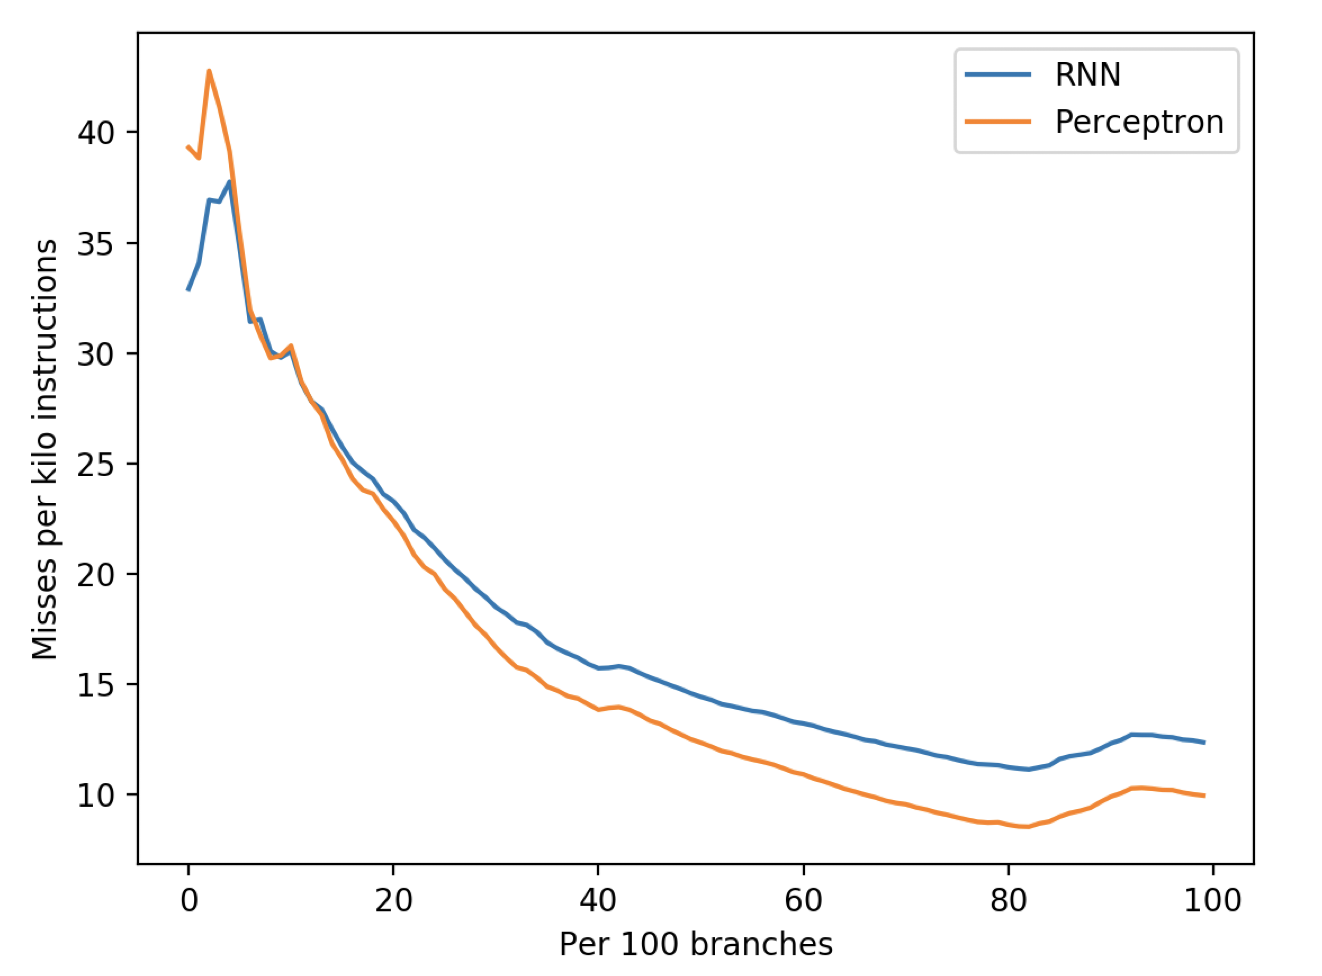
\includegraphics[width=0.7\textwidth]{comparision.png}
  \caption{Progression of perceptron and RNN predictors for 10K branches of INT-2 Benchmark.}
  \label{fig:comparision}
\end{figure}

\section{Conclusion}
It is evident from the results that for a branch prediction problem formulated as an online learning problem, perceptrons are slightly better than RNNs. On a qualitative analysis of the the training progression in \ref{fig:comparision},the kinks would correspond to new program constructs such as entering a nested loop. It can be seen in the plot that perceptron reacts faster to those constructs compared to RNNs which might be causing the overall loss in accuracy. It also has to be noted that this project does relative comparison of perceptron and RNNs and the actual hardware implementation of these network would be more involved. For example, floating point weights in hardware are not practical and as result actual hardware implementations would have to find integer approximations of these networks like those found in \cite{Jimnez2000DynamicBP}.

\bibliographystyle{unsrt}
\bibliography{refs}

\end{document}